\chapitre{La fille sous la lanterne, le jeudi 28 juillet 2033 }{Toute la nuit,}{ Timothée rêve de manœuvres militaires. Ici une légère avancée avec attaque par le flanc droit, là un repli stratégique avec récupération de deux lance-flammes, encore ici une infiltration en pleine nuit de la ligne ennemie, le couteau entre les dents, et là, un enfouissement précipité dans le sol sablonneux. Le colonel Robespierre Alcide est partout en train de dicter des ordres dans son microphone de casque, de pousser sur des traînards aux yeux hagards, de chapitrer ses subalternes immédiats, de s’adonner au cliché cinématographique du genre «ils font quoi les connards de l’aviation ?» ou «pourquoi c’est toujours ma pomme qui hérite de la pire bleusaille ?» ou «il va falloir rapporter des dommages collatéraux !». Des tirs de mortiers ajoutent à l’ambiance sans faire de dégât, des fusées éclairantes couvrent de magenta orangé le terrain de manœuvre, des nuages de fumée à forte odeur pour abréger la souffrance de ses frères : morphine en injection, air comprimé et tout le cirque.  }

Sans se soucier du métal qui hurle à des vitesses folles au-dessus de lui, charriant parfois une tête, une jambe, une épaule, le brancardier Tardif saute de trou en trou. «Faut que tu bouffes», lui crie, confortablement assis dans le sien, Shimoune Saint-Pierre, caporal d’intendance, en lui lançant un carton non recyclable de Nutrisuz. Mais soudain, le sergent Tremblay, Marie-Odile de son prénom, saute dans leur planque. « Qu’est-ce que vous foutez ici en train de bouffer, mes salauds ? On s’entretue là-bas ! Votre compte est bon !». Mais au moment où elle bondit pour retourner au casse-pipe, un shrapnell lui arrache la moitié gauche du visage emportant avec lui la majeure partie du cerveau. «Elle pourra plus nous faire fusiller», fait remarquer Shimoune en mâchouillant, pour le principe, une bouchée de manger mou. «Le Motté, c’est à toi !», lui hurle Ronnie Ross troué de balles, mais encore accroché à sa sulfateuse .50. Timothée rampe jusqu’au moribond, le dégage de la lourde mitrailleuse et, les yeux sur l’inutile collimateur, commence à faire feu des deux poignées.

\begin{floatingfigure}[l]{50mm}
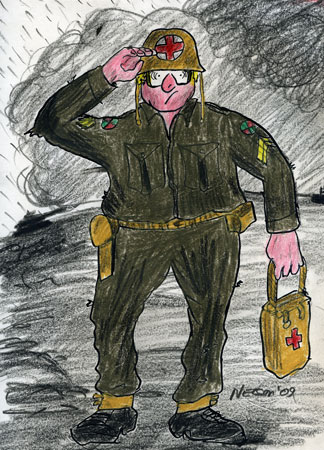
\includegraphics[height=60mm]{corps/chapitre18/img/personnage-timothee-guerre.jpg}
\end{floatingfigure}

Loin en avant, une silhouette se dessine dans la brume et avance dans la pestilence. «Arrête, Timothée-Milet ! Arrête ! On a gagné !», C’est sa mère, la Maririou, archet en main, mais sans son violoncelle. Pataugeant autour d’elle, Gazou a une main arrachée entre les crocs, la main d’un malheureux que les troupes du gros Turcotte ont déchiquetée. «Attention, maman, faut que je tire !». Mais elle continue d’avancer avec sa sale bête, les rafales de .50 lui sifflant à deux millimètres du casque. « Arrête Timothée, arrête, elle t’aime !». Le mitrailleur à la croix rouge s’étire le cou et aperçoit Béatrice en grand uniforme de major, les médailles faisant clinc-clinc. «Béatrice, je ne suis pas un fantassin, je suis un paramédic ! Sors-moi d’ici ! Si tu le fais pas, je vais mourir.» Et la belle l’aide à se lever et, comme si un écran antimétal avait cuirassé la lumière de son aura, l’entraîne sous sa protection vers l’arrière.

Puis il se réveille. En sueur ! Il est 4h45 et déjà certains oiseaux, possiblement les plus affamés ou les moins bien juchés, ont commencé à chicaner l’aurore qui tarde à lancer son travail de mise en lumière. Il ouvre silencieusement sa porte et constate que la rue Crouet sert de canal à une délicate brise bien tempérée par la chaleur des terres plus au sud. Décidément, les temps sont d’une clémence jamais vue. Rien à voir avec les étés précédents o`1 il a surtout éyé question de pluie, d’orages, d’averses et d’inondations. 4h45 ! Plus de sept heures à tirer avant qu’il ne se rapporte, ici même, au colonel Alcide pour les manœuvres devant débuter à midi. Il en sera ainsi pour Claude, Marie-Odile et Shimoune, lequel s’est fait remplacer par Ophélie Marcotte pour la journée. Trop tard pour reculer.

Un chanson lui revient à l’esprit quand il referme sa porte pour s’en aller à la douche.

    Vor der Kaserne
    Vor dem großen Tor
    Stand eine Laterne
    Und steht sie noch davor
    (Devant la caserne
    Quand le jour s’enfuit,
    La vieille lanterne
    Soudain s’allume et luit.)

Le pire, c’est qu’une heure plus tard, en franchissant à pied les quelque cinq kilomètres le séparant du Centre, «Wie einst Lili Marleen», celui de la voix chaude de Marlene Dietrich, lui restera collé dans le creux de l’oreille tout au long de sa balade et même plus. Il aura beau s’efforcer de ne penser qu’au plus horrible de ses cauchemars, il ne pourra s’en débarrasser. Même quand Jawad Kebbaj stoppera son taxi près de lui au début de la rue Sirois.

- Mais qu’est-ce qui se passe, mon jeune homme ? On affame le petit commerce, on n’utilise plus les services du vieux Jawad ?

- Bonjour monsieur Kebbaj. Je profite du beau temps pour marcher jusqu’au travail.

- Tu fais bien, c’est bon pour ta santé, tu fais bien. Tu vas vivre plus longtemps et rester mon client plus longtemps, Masha’Allah !

Quand à 6h15, il arrive «vor des Kaserne», c’est-à-dire devant le Centre, pas un chat ne bouge, personne ne se montre le bout du nez. Seuls des goélands en bande anarchique animent le décor. Mais à l’intérieur, la vie commence à donner des preuves qu’elle bat vraiment. Surtout quand il se pointe au 5e étage où Octavio Torres, un préposé de nuit, l’accueille avec la circonspection d’un douanier de Tijuana en présence d’un visiteur de San Diego.

- Hola Senor Jefe, una gran desgracia … votre bénéficiaire, Jean-Roch Savoie, le lit no 8 de votre SP, il a fait du bordel une partie de la nuit et il est mort tout à l’heure. Il a empêché tout le monde de dormir. Hijo de puta !
L’Illuminé a donc passé l’arme à gauche. Mort faute de traitements significatifs. Mort d’ennui, de déception, de frustration et de rage.

- Merci monsieur Torres, je vais m’en occuper.

Pour l’instant, il n’y a rien à faire, les préposés du grand frigo n’arrivant au boulot qu’à 8 h. Dans la salle palliative, la grogne de ceux qui en sont encore capables est à son comble. Timothée fait le tour de ses grabats pour essayer de calmer ce qu’il peut et s’arrête devant celui de Jean-Roch Savoie, l’homme qui connaissait sa Bible par cœur. Il s’approche du cadavre et, ramassant drap et couverture éparpillés comme à la suite d’une tornade, l’abrille respectueusement et lui joint les mains sur le livre saint qu’il a retrouvé sous le lit. J’ai d’l’argent pour toi, mon garçon.

La voix est celle d’un paquet d’os que plus personne ne lave et qui gît dans la couchette voisine.

- Dormez, monsieur Logan, il n’est pas encore 7 h.

- Je te vire 750 piastres, siffle le pitoyable vieillard, si tu me débarques de la prochaine cérémonie.

Timothée a soudainement envie de hurler, de donner de grands coups de pied dans la fourmilière.

- Écoutez-moi bien, monsieur Logan. Tant que je serai là, y a personne qui va vous amener à la cérémonie. Personne ici n’ira à la cérémonie. Il y en aura p’us de câlisse de cérémonie, c’est-y clair, ça ?

- J’te dis que j’ai 750 piastres …

Comment rassurer ce moribond qui, à juste raison, est convaincu que seul un pot-de-vin peut lui rallonger sa vie de quelques semaines ? Comment l’amener à croire que la pratique des cérémonies gaz létal - sac noir - chariot sera abolie dès que le colonel Alcide aura gagné la guerre ?

- Oubliez la cérémonie, monsieur Logan, y en aura plus, plus jamais, lui répète-t-il en se sauvant.

À son étonnement, le système informatique semble fonctionner. Vlado Marcovsky a-t-il fait des miracles ou est-ce là un effet du hasard ? Il va donc en profiter pour essayer de ne plus penser au rendez-vous de midi, pour tenter de se débarrasser de Lili Marleen qui lui squatte l’esprit et pour liquider tout le retard administratif accumulé depuis une dizaine de jours. Ainsi, il ne voit pas le temps filer et est presque étonné quand Ronnie Ross et Steve Grenier se pointent, dix minutes en retard, pour commencer leur quart.

- T’es d’bonne heure à matin, Motté ? s’exclame Ross.

Le chef de section fait un léger signe de tête et leur annonce la mort de Jean-Roch Savoie.

- Je viens d’appeler au frigo, ils arrivent. Ça me prend quelqu’un pour faire le nécessaire. Tu veux t’en occuper, Steve ?

Le gaillard accepte sans rouspéter et disparaît avec son collègue-comparse, tandis que le téléphone couine pour être pris en charge.

C’est le docteur Prévost, le médecin légiste qui est sur l’affaire Robert Gagnon. Le toubib a le verbe pédagogique, celui de l’expert qui sait que l’être humain ne comprend généralement rien à rien. S’il appelle, insiste-t-il, c’est que son ami le docteur Bellavance le lui a recommandé. D’entrée de jeu, il dit avoir une idée précise des causes et des circonstances ayant pu causer la mort de Dart Vader et estime que le dossier devrait être transféré à un coroner enquêteur. Rien de moins !

- Euh, il est mort de quoi … ?

- D’un choc anaphylactique aux alentours de 23 h lundi soir.

- Une réaction allergique, euh…, exacerbée …

- Oui. Je vois que vous vous y connaissez un peu.

Et le bon docteur de cliquer sur Médecine 101 avec le ton, le débit et la méthode, sans toutefois exiger que l’on prenne des notes. Le choc est une manifestation d’hypersensibilité immédiate due à un allergène, commence-t-il. En fait, le processus est d’une logique implacable. Pour réagir à la présence de l’allergène, le système libère des médiateurs vasoactifs bien connus, des substances comme l’histamine, la sérotonine, les prostaglandines, les leucotriènes, et de tout leur cortège de misères qui entraînent non seulement l’écrasement des systèmes de résistances vasculaires périphériques, «ce qui, monsieur Tardif, peut générer une hypovolémie relative», mais aussi une augmentation de la perméabilité des capillaires, ce qui, à son tour, «peut causer une hypovolémie absolue et de l’œdème».

- Le patient commence à mal aller …

- Exactement, monsieur Tardif. Le cœur tente de compenser en augmentant son rythme dans le but d’éviter une chute de la pression artérielle. Mais ça foire et on assiste rapidement à un collapsus cardio-vasculaire.
Prévost est affirmatif. Pour lui l’affaire est entendue. Deux causes peuvent expliquer le décès du vieux Dart. Tout d’abord, un arrêt circulatoire a fait pomper le cœur à vide ce qui a provoqué son arrêt, «un peu comme une pompe qu’on désamorce». Ensuite, la malignité de l’allergène a causé, au même moment, de la spasticité au niveau du système respiratoire …

- Ce qui l’a asphyxié …

- Il n’a eu aucune chance, ponctue le médecin légiste.

- C’était quoi l’allergène ?

- Les crevettes.

- Il en avait plein la bouche …

- C’est ce qui m’amène aux circonstances.

Et voilà l’homme de science reparti. Robert Gagnon, continue-t-il, est un personnage connu pour s’être adonné toute sa vie aux plaisirs de la bouffe bien arrosée. Or, depuis trois ans, il est exclusivement au régime Nutrisuz. On parle d’un patient dont le dossier médical ne fait état d’aucune allergie. Eut-il éprouvé des difficultés à manger des crevettes ou autres dérivés iodés, on l’aurait su. On peut donc présumer qu’au moment où le dossier a été complété, il pouvait avaler des crustacés sans aucun effet secondaire. Pourtant, il a subi son choc anaphylactique fatal après avoir absorbé, «de par ce que j’ai pu mesurer dans l’estomac, monsieur Tardif», une quantité de nourriture qu’on pourrait qualifier «d’abus du temps des fêtes», mais sûrement pas «d’orgie alimentaire». Il y avait un peu de tout, dont, en dernier, des crevettes. Bref, les circonstances de sa mort sont limpides : Robert Gagnon s’est introduit sans autorisation dans des locaux où on avait entreposé de la bouffe et s’est mis à bâfrer. Arrivé aux crevettes, il est mort d’un choc anaphylactique et n’a pas pu aller plus loin dans son projet, «s’il en avait un». Ce qui signifie qu’entre son admission au Centre, il y a trois ans, et ses frasques de lundi soir, Gagnon a développé une intolérance majeure aux crevettes et, probablement, aux autres dérivés iodés.

- La question est maintenant de savoir pourquoi. Y a-t-il un lien avec le régime au Nutrisuz ? C’est une piste qui, avouons-le, est très séduisante. Et, tant qu’à soulever cette hypothèse, y a-t-il d’autres cas au Québec ? D’où mon intention de transférer le dossier à un collègue coroner enquêteur. Qu’en pensez-vous ?

Timothée est très impressionné.

- À votre connaissance, monsieur Tardif, Robert Gagnon mangeait-il autre chose, vous savez cette nourriture qui leur arrive par voie de contrebande ?

- Sûrement. Mais on parle toujours de nourriture sèche, de cochonneries, bonbons, chocolats, et ainsi de suite, des trucs qui se camouflent pour éviter d’être repérés aux contrôles. En trois ans, on n’a jamais intercepté de vraie nourriture, en-tout-cas pas de crevettes ou de fruits de mer.

De grands pans de mur ne cessent de tomber autour de Timothée. Après le docteur Bellavance qui est prêt à collaborer pour dénoncer le trafic d’hormones, après la découverte de Shimoune Saint-Pierre sur laquelle le commando Alcide va frapper tout à l’heure, après l’agent de sécurité Tropecolo qui serait, affirme Marie-Odile, en train de monter un dossier sur les pouvoirs abusifs d’incarcération dont jouit le tandem Michaud-Dauphin (incidemment, qu’arrive-t-il du bonhomme Jean accusé de sabotage de Saguewanish ?), après le docteur Gagnon dont les dents ont toutes été arrachées grâce à un savantissime petit enregistrement numérique, voici maintenant une enquête du coroner sur les conséquences de cet abominable régime au Nutrisuz. Autant de portes ouvertes qui n’existaient pas il y a une semaine. Des portes qui mènent directement aux terriers du gros Turcotte, de Pete Barrett, de Carl Michaud, de Philippe Dauphin et de bon nombre de leurs collaborateurs. Or, se dit Timothée, il a lui-même, personnellement et activement, participé à l’ouverture de toutes ses portes, lui le binoclard en chauvaison dont la bedonnance dondaine ne l’aide sûrement pas à plaire aux femmes, à plaire à Béatrice. Et, qui sait, si tout marche comme le prévoit Robespierre, cet impavide colonel Alcide, il n’y aura plus jamais de vieux provisoirement vivants qui seront gazés pour satisfaire aux exigences administratives du gouvernement. Peut-être que le père Logan n’a finalement rien à craindre. Et, qui dit Logan, dit Luce Morency, créature inoffensive à la merci des malfaiteurs qui sévissent le 6e Nord, malfaiteurs en lice pour une amère défaite militaire.

    Vor der Kaserne
    Vor dem großen Tor
    Stand eine Laterne
    Und steht sie noch davor 

À 11 h 30, il est encore sous l’effet du musicrobe allemand quand il quitte son officine pour gagner l’antre de Robespierre, un antre qu’il découvre aussi à l’ordre qu’un satellite haut de gamme de la bibliothèque des Ursulines.

- Madame Bellow a terminé son nettoyage des écuries d’Augias ?

- Oui, mais j’me retrouve plus !

- On y va ?

- Ouais, je viens juste de finir mon plan, répond-il en brandissant un grand carton blanc dessiné et colorié à la main comme au temps de l’école élémentaire. Tu veux amener le lutrin et la canne pointeuse, là ? Marie-Odile nous attend dans le stationnement. Let’s go !

Le trio arrive sur la rue Crouet presque en même temps que Shimoune Saint-Pierre. Claude Sey est déjà en train de humer l’air de Nazareth, nonchalamment appuyé sur sa bagnole, et ne semble pas nerveux. En face, Richard n’est pas à sa fenêtre. De toute façon, tout le monde s’en fiche !

%\begin{floatingfigure}[l]{30mm}
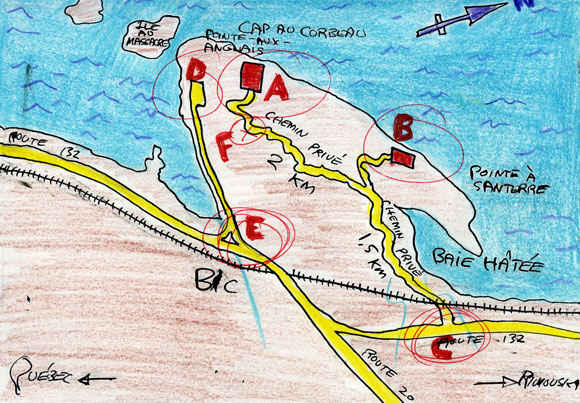
\includegraphics[height=80mm]{corps/chapitre18/img/carte.jpg}
%\end{floatingfigure}

Robespierre a vite fait d’installer sa panoplie du petit généralissime dans le salon et, minutieux, il se met en devoir de réarticuler tous les détails de son plan d’intervention. Le commando partira avec deux voitures. Dans la première, celle de Shimoune, les quatre hommes prendront place et, dans la seconde, une auto-patrouille officielle bien identifiée à la Sécu, Marie-Odile sera seule. Shimoune restera sur la 132 jusqu’au Bic, et bifurquera vers la droite à l’intersection menant à la pointe aux Anglais.

- Ici à «E», tape-t-il de sa canne.

Le préposé au Nutrisuz réprime in extremis le besoin de pouffer de rire.

- De là, on parcourt environ un kilomètre et on stationne ici à «D». Y a toujours de la place. On verrouille et on suit Shimoune dans le bois qui nous amène en vue de l’objectif représenté ici par la lettre «A». Pas besoin de machettes, c’est assez dégagé. On demeure embusqué sans grouiller ni parler jusqu’à 14 h. Pendant ce temps, continue le stratège, Marie-Odile quitte la 132 à la Baie-Hâtée, lettre «C», et emprunte un chemin privé. Il n’y a aucune barrière. Elle roule jusqu’à sa position d’attente et n’en bouge pas avant 13 h 58. Personne n’est censé la voir. C’est ici, lettre «F». À 13 h 58, elle redémarre et, à 14 h, elle commence à faire du bordel avec son auto-patrouille devant l’entrée. Normalement les deux gardiens vont s’approcher pour savoir ce que la Sécu vient faire dans leur petit paradis perdu. Jusqu’ici ça va ?

- Ça va ! répond-on en cœur.

- Nous autres, les gars, à précisément 14h, on fonce vers le pavillon et on l’investit.

Shimoune lève la main.

- Y s’passe quoi si Marie-Odile n’est pas arrivée ?

- On va le savoir, on ne l’entendra pas faire son bordel. On va simplement patienter jusqu’à ce qu’elle se pointe le bout du nez. Mais ça ne se produira pas. N’est-ce pas Marie-Odile ?

La femme flic se contente de sourire.

- Le fait de pénétrer dans la maison va attirer l’attention des deux gardes et ils vont faire deux choses. Ils vont courir vers nous pour voir ce qui se passe et, en même temps, ils vont téléphoner à leur supérieur pour annoncer un incident majeur. Pendant ce temps-là, Marie-Odile vient se positionner sur la galerie avant, juste en haut des escaliers, et elle nous attend, Shimoune et moi. C’est nous trois qui protégerons Timothée et Claude. OK ? Shimoune, rappelle-moi ton rôle !

- Je te suis au pas, mon bel Hannibal, et je viens me faire aller les biceps à côté de Marie-Odile sur la galerie avant. Youhou les amis, venez admirer mes formes voluptueuses ! Mais le premier qui se laisse tenter, je lui casse le nez.

- Espèce d’agace ! OK. Et toi, Marie-Odile ?

- Je descends de mon auto et je gagne la galerie où je vous attends, toi et Shimoune. Le premier qui approche, je lui pète les dents.

- Ouille ! Et toi Timothée-Milet Rioux-Tardif ?

- Je te suis dans la cour, j’attends que tu ouvres la porte d’en arrière ou que tu la défonces si on l’a verrouillée, j’entre à mon tour et je fonce vers la droite où je filme tout ce que je vois en mode téléversement actif – c’est la petite lumière bleue qui clignote. Mon objectif ? Les deux Turcotte.

- OK ! Et notre jeune ami, monsieur Sey ?

- Même chose que Timothée, mais moi je fonce vers la gauche. Dites, monsieur Alcide, il arrivera quoi de l’appel à l’aide que feront les agents qui nous verront attaquer le pavillon ?

- L’appel sera reçu directement chez Barrett à cinq minutes d’ici. C’est la lettre «B». Comme c’est le haut lieu des basses œuvres de l’organisation Turcotte, il s’y tient toujours des activités partisanes. Ce qui m’incite à croire qu’il y a, en tout temps, des fiers-à-bras en attente de casse. C’est comme ça que ça marche. J’imagine qu’ils vont venir avec une ou deux voitures, c’est-à-dire avec deux ou quatre gorilles que Marie-Odile, Shimoune et moi devrons neutraliser. Le plus vite qu’ils peuvent arriver c’est cinq minutes après notre petite invasion domiciliaire. Mais cinq minutes c’est amplement suffisamment pour que Timothée et vous, monsieur Sey, puissiez filmer la cible et téléverser vos enregistrements vidéo dans le serveur sécurisé de la Sécu, au Centre. Dès lors, les méchants seront foutus et, s’ils tiennent malgré tout à la bagarre, ils la perdront, n’est-ce pas Marie-Odile, n’est-ce pas Shimoune ? De toute façon, elle sera légalement retenue contre eux. Rassuré, monsieur Sey ?

- B’en, si c’est ce qu’il faut faire pour recommencer à traiter les personnes âgées avec un peu de dignité, à cesser de les considérer comme des animaux indésirables, pour leur ouvrir toutes grandes les fenêtres sur la vie, les jeunes, la nature, le vent du fleuve, la joie de vivre, ma réponse, monsieur Alcide, moi le p’tit cul de 28 ans, c’est que oui, ça va et que je suis fier d’en être.

- Parfait ! Madame, messieurs, il ne nous reste plus qu’à synchroniser nos montres.

Mais depuis un bon moment, Romain est en bas, au pied de l’escalier, et, très inquiet, il essaie de savoir ce qui se trame chez son fils. À sa connaissance, c’est la première fois qu’il s’y trouve autant de monde en même temps. Qui plus est, de jour ! Pour mieux arriver à comprendre, il a même déposé Gazou, manu militari, sur la corniche entre poules et lapin. Sans bouger, il prête l’oreille, soucieux de déchiffrer les bribes de conversation qui lui parviennent. Voilà maintenant que c’est le carillon d’entrée qui se fait entendre, suivi de pas, de paroles vagues, puis encore d‘autres pas qui, cette fois s’approchent de l’escalier. Rapidement, le vieil homme regagne son salon.

C’est Béatrice qui apparaît dans le cadre de la porte. Elle avait effectivement promis la veille de passer visiter Marie en début d’après-midi. Oui elle a eu le loisir de voir les gens qui sont en haut, non elle ne sait pas de quoi ils discutent, bien qu’elle ait remarqué un plan affiché sur un lutrin, et non elle ne les connaît pas tous.

- Y a un blond bizarre avec des bras musclés et un plus jeune, une espèce d’intello pas souriant. Les autres c’est Timothée, notre ami Robespierre Alcide et une agente de sécurité du Centre, Marie-Odile Tremblay.

- Y s’passe quelque chose en haut, ça, c’est sûr.

La Maririou ouvre de grands yeux.

- Voyons Romain, que ch’est que tu veux qui’ch pache ?

Convaincu de devoir insister, Romain présente la synthèse de ce qu’il a perçu, enrichi de ce que Béatrice vient d’ajouter. Cinq personnes réunies chez Timothée sont en train de parler très sérieusement – «y a même un agent de sécurité avec eux» - de s’en aller filmer les parents du gros Turcotte dans leur cachette. Ils savent où aller et ils ont un plan d’attaque.

À l’extérieur, Gazou hurle à la mort, ce qui affole les poules et angoisse les lapins. Sans parler des résidents de la rue. Marie se lève, une étrange lueur dans les yeux, et va faire entrer l’affreuse bête. En apercevant Béatrice, le cabot ravale sa hargne et son hostilité pour aller se prosterner en face d’elle dans le plus mystique des silences.

Le gros Turcotte ! Le pouvoir des colosses aux voix rauques, grasses et tonitruantes, aux mains énormes, velues, tachées de nicotine, encroûtées de malfaisances, des mains animales, primitives, exécutrices qui égorgent les écoles de musique, qui frappent les petites filles de onze ans, qui détruisent les vies, qui institutionnalise l’échec dans la suite des choses.

- T’es chertain que che chont les parents du gros Turcotte ?

- C’est ce que j’ai entendu à quelques reprises.

Si les jeunes, en haut, ont décidé d’agir ainsi, ce n’est probablement pas pour le plaisir de faire de l’exercice. Il faut plutôt imaginer, puisqu’il est question de parents illégalement cachés, que la manœuvre projetée est en rapport avec eux, Romain et Marie, deux vieux trop avancés en âge pour qu’on songe seulement à leur en parler. Timothée veut-il essayer de faire chanter le ministre pour leur négocier une meilleure qualité de vie ? Si cela est possible, le plan, quel qu’il soit, les concerne. Cela ne risque-t-il pas de changer leur vie, en mieux ou en pire ? De toute façon, les choses ne peuvent aller plus mal que maintenant; il faut agir !

- C’est choquant qu’ils ne nous consultent pas, on n’est quand même pas encore rendu gaga !

- On est loin d’être rendu gaga, mon Romain ! S’ils jont trouvé les géniteurs du gros verrat, faut que je chois là, faut que je l’attrape le gros malfaijant, faut que j’lui coupe ches groches pattes épeurantes pour plus qu’il fache plus de mal à perchonne.

Romain se retient de réagir. Il sait que si sa vieille a une idée précise en tête, il n’y a plus rien à faire.

- Comment tu vas faire ça ? risque-t-il.

En trois mots secs, elle explique que s’ils montent au rez-de-chaussée, tous trois, là maintenant, Timothée et sa bande ne voudront jamais les intégrer à leur équipée. À coup sûr, ils vont justifier le danger de l’opération, l’état de santé de Marie, le tour de taille de Romain, la convalescence de Béatrice, voir l’alignement des planètes rendant impossible toute mission de plus de cinq exécutants. Il faut donc trouver une façon de participer à la fête sans attendre d’être invités.

- On écoute che qui che pache en haut et quand on les jentend partir, on che dépêche et on les chuit dans le char à Béatriche. T’as-tu un meilleur plan ?

Romain bouge la tête à l’horizontale et regarde Béatrice qui hausse les épaules en souriant.

- Bon ! J’m’en vas me préparer.

Cinq minutes plus tard, elle ressort de sa chambre en robe fleurie jaune, verte, noire et blanche, avec collants gris et souliers vernis, toute coiffée comme pour la messe de minuit, tenant, dans sa main gauche, un parapluie. Constatant les regards dubitatifs sur son accessoire conçu davantage pour le crachin atlantique que pour les chaudes après-midi de juillet, elle leur en donne l’explication.

- Perchonne au monde ne bloque le chemin à une p’tite vieille qui a l’air de chavoir manier un parapluie.

Suit alors une courte période d’attente qui se termine par un branle-bas de combat au-dessus de leurs têtes.

- Cha y est !

Ils perçoivent clairement une voix de femme s’écrier qu’elle va suivre avec sa voiture. Suivre qui ? Sûrement Timothée et les autres gamins. Plus une seconde à perdre ! Béatrice et Romain commencent à monter tandis que Marie ferme la porte au nez de Gazou, «Moman part pas longtemps, chois gentil !», lequel, aussi con qu’un pot de beurre d’arachides, se remet à hurler comme si la fin du monde était arrivée. La contemplation de Béatrice entraînerait-elle un état de dépendance et son manque, une souffrance intolérable ?

- Envoye, Romain, t’as donc b’en d’la misére à grimper les marches !

- J’ai p’us vingt ans !

Béatrice se précipite vers la porte.

- Dépêchez-vous, elle vient de décoller.

En ahanant, Romain parvient à l’auto où la Maririou est en train de s’attacher sur le siège avant. Il a à peine le loisir de s’asseoir que déjà, Béatrice a embrayé et que l’hybride chinoise fonce en direction ouest. Rue La Salle, elle entrevoit, au loin, le véhicule de la Sécu qui vient d’arrêter au feu rouge du boulevard Saint-Germain.

- On l’a rattrapée !

Le reste de la filature est sans histoire. Trois cents mètres prudemment en arrière, Béatrice a le temps d’apercevoir Marie-Odile quitter la 132 à la Baie-Hâtée. Comme on ignore où ce chemin privé mène, le mieux, estime Romain, est de l’emprunter et de voir. Au pire, l’agente de sécurité les remarquera et viendra les houspiller. Au mieux, ils la suivront, invisibles, jusqu’à sa destination.

Peu après, ils passent devant une ramification secondaire qui semble conduire à une propriété cossue dont on entraperçoit quelques détails évanescents au travers les arbres. Dans le pare-brise, la petite route en gravelle serpente cahin-caha et bloque toute perspective de plus de 100 mètres, tant et si bien que la conductrice doit redoubler de prudence pour ne pas être repérée.

Après cinq ou six minutes de reptation à bas régime, l’infirmière aperçoit, de loin, ce qui pourrait être la voiture de la Sécu immobilisée et elle ferme son moteur. Son rythme cardiaque a augmenté de façon perceptible.

- Qu’est-ce qu’on fait si elle fait demi-tour ?

- On a l’air fou, ronchonne Romain. Mais on dirait qu’elle attend quelqu’un ou quelque chose.

- Je vais aller voir. Vous autres, restez pas dans l’auto. Si jamais quelqu’un vient…

Doucement, on ouvre les portières et on entre dans le sous-bois. Avec toutes les ruses expérimentées au fil des millénaires par l’ensemble des peuplades amérindiennes, les vieux marchent jusqu’à la carcasse d’un tremble recouvert de mousse et Béatrice s’avance en direction de Marie-Odile. Sans faire craquer de branches, elle réussit à s’en approcher à dix mètres où, immobile, elle épie. Rien ne bouge, personne ne vient. Seuls les oiseaux font preuve de vie. Puis, comme si elle obéissait à une consigne, l’agente de sécurité démarre en trombe et disparaît dans les courbes prononcées du chemin. L’infirmière a beau s’étirer, elle ne la voit plus. Hésitant sur la marche à suivre, elle choisit de s’en retourner vers sa propre voiture, mais, chemin faisant, elle entend le moteur de Marie-Odile s’arrêter, une portière claquer et une voix féminine crier des choses qu’elle n’arrive pas à bien comprendre. Elle refait volte-face et continue sa progression dans la lourde couverture boisée. Elle a vite fait de repérer une clairière où elle aperçoit l’auto-patrouille, puis l’agente de sécurité en train de courir vers une grande maison, tandis que deux gaillards, on dirait des gardiens, se hâtent, eux aussi, vers l’arrière de la propriété, la main sur leur système personnel de communication. L’un d’eux invective lourdement la policière, utilisant des termes blessants, l’autre ne cesse de parler dans son appareil. Puis tous deux changent de cap et s’avancent vers Marie-Odile qui, en position dite du «sablier large», le Hangetsu-Dachi, les attend silencieusement en haut des marches de la galerie. La perspective de recevoir des coups les fait hésiter et ils tentent de parlementer. C’est alors que Robespierre et son copain, le gars aux bras surdéveloppés, apparaissent à leur tour; ils étaient dans la maison. Prudemment, les deux gardiens font machine arrière ce qui incite le blond à adopter la pose de Monsieur Univers et à s’agiter la musculature.

- Hé ! les tites filles, dites-moi pas qu’on vous fait peur !

L’un des gardiens lui signifie un doigt d’honneur.

- On a “câllé” du renfort, t’es faite le fif, toi aussi la Bitch !

Ce que Béatrice comprend, c’est qu’une partie de ceux qu’elle a vus tout à l’heure sur la rue Crouet est ici en train de braver des gardiens de sécurité qui ont appelé du monde à la rescousse. Elle ignore où sont les deux autres, Timothée et l’intello, mais elle sait que des gens s’en viennent, possiblement des taupins mal intentionnés, des gens qui vont obligatoirement emprunter le chemin où est approximativement garée sa voiture et près de laquelle patientent présentement deux vieillards. Convaincue du pire, elle saute sur la gravelle et se met à courir en leur direction.

- Restez cachés, leur crie-t-elle tandis qu’elle met le contact pour se stationner sur l’accotement, un bien grand mot pour qualifier la roche grossière mal râtelée de chaque côté du chemin.

Satisfaite de voir ses portières de droite empêtrées dans les premières branches, elle verrouille et se fond dans la verdure où elle vient rejoindre ses compagnons. Malheureusement, elle doit retourner à l’auto, Marie tient absolument à son ombrelle, ce qu’elle fait sans maugréer.

Pendant qu’elle leur raconte tout ce qu’elle a vu au pavillon, des bruits de moteur se font entendre. Tous trois se tapissent et assistent au passage à vive allure de deux voitures trimbalant chacune, quatre casseurs. Aucun ne semble porter attention à l’hybride de Béatrice.

- Ces gars-là, madame Rioux, ils s’en vont à la maison, là-bas, ramasser Timothée et ses amis.

- Là où che cachent les parents du gros Turcotte ?

- Oui.

- J’ignore quelle idée ils jont eue Timothée et ches amis, mais là, che que je vois, c’est qu’ils vont che faire rentrer dedans. Cha va faire ! Je m’en occupe ! En route !

Et la Maririou de quitter le sous-bois pour s’en retourner prendre place dans l’auto.

- Dépêche, crie-t-elle à Béatrice.

- Voyons madame Rioux, ça n’a pas de bons sens ce que vous voulez faire là !

- Vite, gronde Romain en se hâtant à son tour vers le véhicule, fais ce qu’a te dit, elle sait ce qu’elle fait !
Mais au même moment, les choses se gâtent au pavillon. Aux deux gardiens se sont ajoutés huit videurs armés de matraques et possiblement d’armes à feu, qui s’approchent de la galerie où Robespierre, Marie-Odile et Shimoune jouent les matamores. De l’intérieur, la voix de Timothée se fait entendre :

- C’est beau, Robespierre, on a tout. Mission accomplie !

\begin{floatingfigure}[l]{45mm}
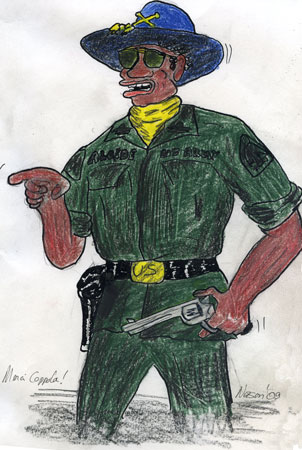
\includegraphics[height=60mm]{corps/chapitre18/img/personnage-robespierre-colonel.jpg}
\end{floatingfigure}

Le colonel Alcide sourit ! Jusqu’ici, sa stratégie a fonctionné. Sauf que, devant lui, la perspective est moins enthousiasmante. Il va maintenant falloir en découdre avec deux fois plus de salopards que prévu.

C’est Marie-Odile qui se lance dans les frais, une improvisation par rapport au plan initial, une improvisation heureuse.

- Écoutez-moi bien, gang de bolos. Nos gars en dedans ont filmé tout ce qu’ils étaient venus filmer et ils en ont téléversé une copie dans le serveur de la Sécu au Centre. Nous avons maintenant toutes les preuves que nous voulions. Pour détruire ces documents, ça va prendre un ordre de la Cour. À c’t heure, vous avez le choix. Vous venez nous chercher ou vous nous laissez filer sans violence.

Un peu en retrait des autres, un des sbires de Pete Barrett ne cesse de parler dans sa boucle d’oreille, ce qu’il fait avec force gestes sans trop s’occuper de ses collègues qui eux, semblent plutôt décidés à déloger les occupants de la galerie.

- Tout ce que vous faites présentement est filmé et archivé, continue la femme flic en pointant sur le premier bouton de sa chemise. Utilisez vos guns et vous serez poursuivis pour tentative d’homicide.

- Ta gueule, astie de Bitch, crie un des malabars. Let’s go, les boys, on les défonce !

Et les affreux de se mettre en branle. L’intensité est à couper au couteau. Dans quelques secondes, les coups vont pleuvoir. C’est précisément à ce moment qu’arrive, à file épouvante, la voiture de Béatrice, laquelle vient de franchir sur les chapeaux de roues trois croches et une montée à pic. Sans hésiter, la Maririou en descend et, pointant du riflard, fonce de son pas précipité de petite vieille pas commode vers le pavillon. Il faut la voir se faufiler au milieu des malfrats en les tassant avec son improbable accessoire. La stupéfaction est totale. Personne ne la connaît, personne ne l’a jamais vue, ni les méchants qui n’osent se placer sur son chemin, ni le trio en position défensive sur la galerie qui la laisse monter. Mais c’est Romain qui est encore le plus impressionné. Il sait parfaitement bien que toute sa vie, sa belle Marie a eu peur des hommes violents et la voilà en train de les bousculer à la manière de volailles dans un poulailler.

- Bonjour madame, à qui ai-je l’honneur ? lui demande Robespierre.

- Laiche faire les jonneurs, toi ! Ouvre-moi la porte !

Et elle s’introduit dans le pavillon.

Dans sa foulée, Romain et Béatrice tentent d’avancer. Mais deux gredins ont tôt fait de les intercepter, un peu comme s’il était hors de question qu’on leur refasse le coup de la vieille dame au parapluie.

Ce que voyant, Marie-Odile hurle de plus belle.

- Tout est filmé !

Intimidé, le gorille qui retient Romain le relâche aussitôt, mais son collègue hésite à en faire autant avec Béatrice. Distrait dans son incertitude, il ne voit pas venir le coup de genou dans ses parties normalement intimes. C’est en geignant qu’il entend cette belle fille rajouter une kyrielle de grasses insultes à sa sourde douleur et qu’il la voit prendre la main du vieillard pour l’amener en direction de l’immeuble. Sur la galerie Marie-Odile a presque souri.
Aussitôt entrée, la Maririou remarque Timothée qui vient vers elle, la regardant incrédule, comme s’il eut vu apparaître Bea Bellow armée d’un lance-roquettes. Puis, juste à côté, elle aperçoit la personne qu’elle cherchait, une forte femme d’allure austère qui semble très contrariée par la situation générale.

- Mimi Turcotte, t’es pas chensée être morte il y a quatre ans, toi ?

- P’is toi, Marie Rioux, t’es pas censé l’être depuis six ?

Toutes deux se dévisagent comme si elles s’accusaient d’avoir raté un soufflé.

Derrière la mère Turcotte, quelques vieillards se sont approchés dont son époux Jean-Pierre, une montagne de chair vaguement connue de Romain, Romain dont les yeux haineux fixent ces illégaux financés par la princesse, ces vernis torchés blanchis par le pouvoir libéral, ces planqués aux panses replètes gavées par les contribuables. Et il explose. Voilà six ans que lui et sa compagne sont enfermés dans un sous-sol qui sent la crasse en raison d’une loi inique que le fils Turcotte a fait voter et a mise en place. Et pendant ce temps-là, pendant qu’il faisait crever des milliers d’aînés dans des CRG mal équipés, pendant qu’il en condamnait un plus grand nombre à la clandestinité, à la non-existence officielle, à la peur, aux privations, aux abus de toutes sortes et aux souffrances, une petite clique de gras dur, son père et sa mère en tête, menaient un train d’enfer propre aux parasites institutionnalisés.

- Romain, arrête !

Ce cri venu du fond des tripes est accompagné par un violent coup de riflard sur la table de la salle à manger. Un vase de fleurs des champs se renverse.

- Ch’est mon affaire. Ch’est moi qu’il a trahie le gros crevard. Toi, il ne t’a fait que chouffrir, comme tous les autres vieux du Québec. Mais moi, en plus et churtout, il m’a abujée.

Mimi Turcotte est effarée et l’obèse à ses côtés n’ose parler.

- Mais avant que tu m’entendes, Mimi Turcotte, tu vas chortir dehors et tu vas dire à tes chiens de retourner dans leur cabane. Je te tiens rechponsable des coups qui vont ch’échanger.

Étrangement, la mégère évite de répondre et gagne la galerie où elle lève les deux bras.

- Arrêtez tout, crie-t-elle aux tueurs. J’ai le contrôle; attendez les ordres de Pete avant de bouger.

Aussitôt dit, aussitôt fait. Les casseurs se replient jusqu’au chemin d’accès, leur chef en grands pourparlers téléphoniques.

Robespierre qui vient de voir son plan complètement bousillé, heureusement bousillé, s’approche de Marie.

- Mon ami Timothée me dit que vous êtes sa mère, madame. Je suis très heureux de vous connaître. Mais venez vous asseoir ici à la table. Faut plus vous en faire, on a le contrôle. On a tout filmé. On a ramassé assez de preuves pour faire dégommer le gros pourri et pour initier un grand ménage au Centre.

Claude Sey semble ravi.

- Pauvre ‘tit garchon, qu’elle répond à l’armoire à glace chocolatée - étrangement, elle n’en ressent aucune crainte - en se laissant conduire jusqu’à la table. Y a quelque chose que t’as pas compris.

Toute sa vie, crache la Maririou, elle s’est réfugiée dans la musique, totalement, hermétiquement, cela pour se créer un univers où les Edmond Rioux ne pouvaient accéder. Elle a cru pouvoir y arriver et a même essayé d’expliquer la méthode à des enfants qui, comme elle, avaient été victimes d’hommes en situation de pouvoir, des agresseurs, batteurs, forts en gueule, gueulards à voix tonitruantes, ivrognes colériques, manipulateurs, violeurs et autres monstres, des hommes terribles à l’origine d’existences impossibles à raccommoder et de petites filles de onze ans perdues à tout jamais. Or, dans cette lignée de misérables, Sylvain Turcotte venait prendre place assez haut dans l’échelle d’infamie. Au lieu de respecter sa parole dans l’histoire de l’École de musique, il avait laissé tomber l’institution quinquagénaire comme s’il eut été question d’un insignifiant projet d’été. Pourtant, il s’était bel et bien engagé auprès d’elle, Marie Rioux. Il avait juré de sortir l’École des difficultés financières qui l’accablaient. Malgré cela, il avait agi en sens contraire, ce qui ne l’avait surtout pas empêché de devenir par la suite encore plus puissant, plus gros, plus épeurant, comme, naguère, Edmond Rioux qui, chaque fois qu’il revenait à la maison et qu’il la battait, lui semblait plus terrifiant que jamais. C’est connu, les salauds grandissent dans l’ignominie. Dans l’esprit de la vieille violoncelliste, son père, cet être détesté qu’elle continue aujourd’hui de craindre dans ses cauchemars, lui a tué sa vie, et Sylvain Turcotte, l’homme fort de Rimouski, qu’elle hait dans une rigueur dénuée d’émotions, lui a tué son projet de vie. Ce sont deux exemples de ce pouvoir anéantissant qui vient, parfois, frapper les petites filles de onze ans, même si elles sont devenues des septuagénaires avancées.

- T’auras beau le faire dégommer, le gros verrat, il va rechter méchant, dangereux, épeurant. T’as-tu compris qu’il fallait lui arracher les dents, lui couper les mains, lui nouer la queue, le rendre dochile comme un chien de perron. Tu pourras alors lui donner des coups de pieds et il pourra pas te mordre !

Le docteur Robespierre qui discerne toute la souffrance de cette vieille vie, se garde bien de répondre. Seule Mimi Turcotte s’essaie.

- Tu trouves pas que tu exagères un peu beaucoup, Marie Rioux ! Ta vie a été une catastrophe et tu veux te venger sur mon garçon !

Béatrice s’est rapprochée et s’est assise sur la chaise voisine de Marie. Par réflexe nerveux, elle lui caresse un instant l’épaule.

- Qui t’a parlé de vengeance ? Pour che venger, il faut être enragée. Moi, Mimi, j’chuis calme. Chereine, même. Je parle cheulement d’administrer une prochédure comme quand on opère une bête puante pour qu’elle ne nous arroje plus ou un cherpent pour qu’il ne nous empoijonne plus. Je vas faire cha pour me faire du bien. Au moins une fois dans ma chienne de vie ! Avant qu’il choit trop tard !

Marceline non plus n’avait pas opéré dans la rage, la vengeance ou l’émotion. Elle avait frappé un animal dangereux qui menaçait sa petite fille de onze ans. Pour la protéger. Pour éviter plus de mal. Pour l’avenir, pas pour le passé.

La suite est inattendue. Tout d’abord, Shimoune vient parler dans le creux de l’oreille de Robespierre. Puis il revient avec un des hommes de Pete Barrett qui, sans une parole, prête sa boucle d’oreille à Mimi Turcotte. L’instant est dramatique. Quelques moments plus tard, l’organisatrice libérale met fin à la communication et regarde Marie.

- T’as gagné ! Pete veut négocier !

Des exclamations de joie fusent ici et là, Claude Sey au bord des larmes et Timothée lourdement silencieux, comme s’il ravalait des litres et des litres de peine contenue. Marie-Odile assène un amical coup de coude dans les côtes de Shimoune. Le colonel Alcide n’a pas le temps de parler que déjà, la générale Rioux a donné ses ordres.

- Avant de négochier, Mimi, tu vas renvoyer chez eux les méchants qui chont dehors et tu vas me garantir qu’on peut tous repartir d’ichi chans que rien ne nous arrive. Rendus chez nous, on va regarder cha et on va te contacter.

Une heure et demie plus tard, Marie et Romain participent à ce qui leur avait été interdit depuis l’été 2027. Assis dans le salon de Timothée, ils boivent du vin et mangent de la pizza en compagnie d’étrangers, des hommes et des femmes ivres de joie et de tension dissipée qui n’ont de cesse de se relayer pour se rappeler les grands moments de l’après-midi.

- Mesdames, messieurs, s’écrie Robespierre.

Le silence se fait.

- Je propose un toast à notre chef, à celle qui a rendu possible cette victoire sans qu’il n’y ait d’égratignure, à quelqu’un que j’ai été fier de rencontrer aujourd’hui, à madame Rioux !

Un concert de bravos et d’applaudissements suit.

Après, lentement, comme si on voulait s’accrocher au plaisir d’être dans le groupe, le commando se démobilise, tout un chacun regagnant son domicile. C’est Marie-Odile qui va offrir à Robespierre de le reconduire à sa voiture dans le stationnement du Centre.

- Faut que j’aille porter l’auto-patrouille.

Timothée sourit et les accompagne à l’extérieur.

- Hé-hé-hé, qu’il fait à son ami.

- Quoi «hé-hé-hé» ?

- Juste «hé-hé-hé».

La brunante est déjà avancée et, pour la énième soirée consécutive, le vent est doux et parfumé. Devant sa maison, près du cimetière, un lampadaire commence à décorer la rue de ses effets de lumière et, sous son halo, Béatrice, sortie tout à l’heure humer l’air des terres, semble attendre un signe de la vie. Béatrice, la fille de la lanterne. Attiré comme un papillon de nuit, Timothée s’approche, atrocement gêné malgré ses trois verres de vin. Quand bien même il tenterait de parler, de dire ce que doit en de telles circonstances, il n’y arriverait pas. Rien ne sortirait et, de toute façon, il ne saurait trouver les mots.

C’est ce qui explique qu’elle lui prend la main.

- Dis rien, Timothée, dis rien, je sais que tu es bon. Reste avec moi.

Maladroitement, il prend place à côté d’elle sous le lampadaire, paradis dont les anges pardonnent les bedondaines, les barniques et les chauvaisons.

    So woll’n wir uns da wieder seh’n
    Bei der Laterne wollen wir steh’n
    Wie einst Lili Marleen
    Wie einst Lili Marleen
    (C’est dans ce coin-là que le soir
    On s’attendait près de la lanterne remplis d’espoir
    Tous deux, Lily Marlène.
    Tous deux, Lily Marlène.)

